\clearpage
\sect{5. Training and rescue}

Play as Nick. Pass seven training events, beat the instructor and graduate. Then enter the occupied building and rescue the hostages. Joe is your rival in the training events that show two competitors.

\begin{enumerate}
\item \textbf{Obstacle course.} Build up speed and cross the finish line before time runs out. Jump over barriers. Jump up to grab the overhead bars, then keep tapping the run button to move along them.
\item \textbf{Firing Range I.} Aim and hit at least \textbf{44} targets. The hit boxes fill as you score.
\item \textbf{Iron Man Race.} Cross rough ground and water before time runs out. Use the directions to steer around obstacles or turn back if you miss a crossing. The left view follows you and the right view follows Joe.
\item \textbf{Firing Range II.} Move from side to side and hit at least \textbf{52} robots. Shoot into their path as they come towards you.
\item \textbf{Arm wrestling.} Build up force by tapping quickly once the bout starts. Winning earns a bonus. Either result takes you to the next event.
\item \textbf{Firing Range III.} Hit at least \textbf{32} magenta targets. A shot at the instructor's silhouette jams your controls until the next group appears.
\item \textbf{Instructor fight.} Knock down the instructor before the clock expires. Watch your energy and his, and close the distance only when you can land a kick.
\end{enumerate}

\begin{figure}[H]
\centering
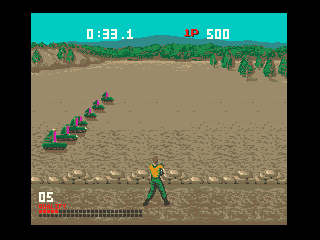
\includegraphics[width=.47\textwidth]{../img/robots.png}\hfill
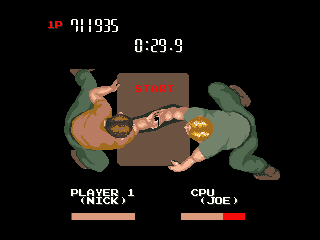
\includegraphics[width=.47\textwidth]{../img/arm-wrestling.png}
\caption{Firing Range II and the start of the arm-wrestling bout.}
\end{figure}

\textbf{Final mission.} After graduation, follow the briefing into the building. Jump onto crates, use overhead pipes, and watch for knives and fire. Clear a path to the final opponent and defeat him to rescue the hostages.

\clearpage
\sect{6. Reading the screen}

\begin{figure}[H]
\centering
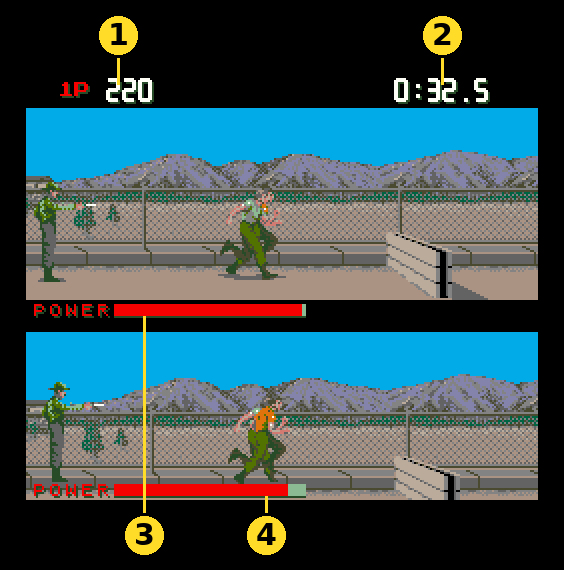
\includegraphics[width=.73\textwidth]{img/race-hud.png}
\caption{The obstacle course. The upper view follows Nick and the lower view follows Joe.}
\end{figure}

\begin{tabularx}{\textwidth}{@{}llX@{}}
\toprule
\textbf{\tNo} & \textbf{\tElement} & \textbf{\tTellsYou}\\
\midrule
1 & \texttt{1P} score & Points earned so far in the run.\\
2 & Clock & Time left to complete the event.\\
3 & Upper \texttt{POWER} bar & Nick's power. Tap the run button to build it up.\\
4 & Lower \texttt{POWER} bar & Joe's power. He is controlled by the computer.\\
\bottomrule
\end{tabularx}

The shooting ranges show the clock, score, sight or line of fire, and a row of hit boxes. In the instructor fight, the energy bars show how much damage each fighter can still take. In the final mission the energy and score display appears during the final fight.

\begin{figure}[H]
\centering
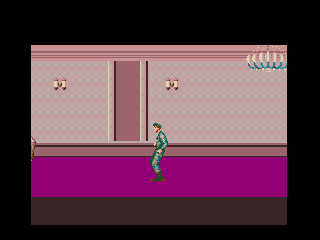
\includegraphics[width=.30\textwidth]{../img/mission.png}\hspace{1em}
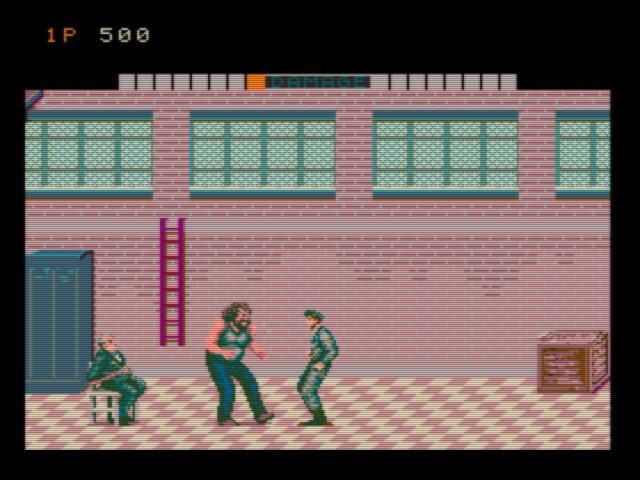
\includegraphics[width=.30\textwidth]{../img/boss.png}
\caption{From the first rooms to the final fight.}
\end{figure}

\clearpage
\sect{7. Second chance and scoring}

\textbf{Pull-ups.} A near miss in either race or any shooting range may earn you one second chance per run. If the instructor sends you to the bar, wait for Nick to grab it, then tap the run button until the counter is clear. Finish in time and you go on without a bonus for the missed event. The arm-wrestling bout does not require a retry.

\begin{tabularx}{\textwidth}{@{}lX@{}}
\toprule
\textbf{Event} & \textbf{Scoring}\\
\midrule
Races & Progress earns points. In the obstacle course, clearing a barrier without climbing earns 500 extra.\\
Ranges I and III & A hit earns 100 to 500 points, depending on its place in the group.\\
Range II & Each hit earns 100 points.\\
Arm wrestling & A win earns 4,000 points and adds three seconds.\\
Instructor fight & A hit earns 500 points. Defeating the instructor awards 100,000.\\
Final mission & Enemies and hits on the boss earn points. Defeating the boss awards 100,000.\\
\bottomrule
\end{tabularx}

Event bonuses add to the same score. Time bonuses shown after training carry over to the indicated next event.

\sect{8. Ranking}

If your score enters the top ten, use the cursor keys or joystick to choose characters. Up or right moves forward through the list. Down or left moves back. Press \key{SPACE} or joystick button~1 to accept. Enter three characters or select \texttt{END}. Scores stay on the table while the MSX is powered on.

\begin{figure}[H]
\centering
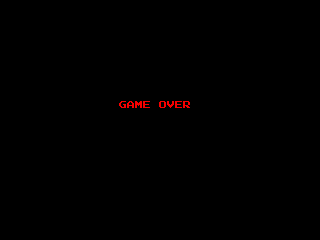
\includegraphics[width=.44\textwidth]{../img/game-over.png}\hfill
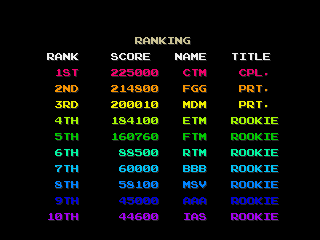
\includegraphics[width=.44\textwidth]{../img/ranking.png}
\caption{Game over and the ranking, with score, initials and rank.}
\end{figure}
